\documentclass[11pt,letterpaper]{article}
\pagestyle{plain}
\usepackage{amsmath}
\usepackage{amssymb}
\usepackage[utf8]{inputenc}
\usepackage{times}
\usepackage{hyperref}
\usepackage{graphicx}
\usepackage{wrapfig}
\usepackage{listings}
\usepackage[usenames,dvipsnames]{xcolor}
\usepackage{setspace}
\usepackage{python_syntax}
\usepackage[sort&compress]{natbib}
\usepackage{bibentry}
\usepackage{todonotes}
\usepackage{url}
\usepackage[compact]{titlesec}
\titleformat{\subsection}[runin]
{\normalfont\large\bfseries}{\thesubsection}{1em}{}
\titleformat{\subsubsection}[runin]
{\normalfont\large\bfseries}{\thesubsubsection}{1em}{}
\usepackage{enumitem}
\usepackage[
top    = 1in,
bottom = 1in,
left   = 1in,
right  = 1in]{geometry}
\usepackage{caption}
\captionsetup{belowskip=0pt,aboveskip=0pt}
\linespread{0.92} % NSF allows up to 6 lines per inch.  
\def\UrlFont{\em} % Italicize all URLs.  
\frenchspacing
\setlist{nolistsep} % or \setlist{noitemsep} to leave space around whole list
\lstset{ %
	basicstyle=\small\ttfamily,
	breaklines=true,
	language=Python,
	}
\let\verbx\lstinline
\newcommand{\bfhead}[1]{\noindent \textbf{#1:}}

% Josh: A lot of the *potential* and actual features of SciDash are
%scattered throughout the document. This gives the reader the feeling
%that its features aren't fully thought out. 

% The lines below are turning underscores into apostophes!  
%\usepackage{alltt}
%\renewcommand{\ttdefault}{txtt}
%\usepackage[scaled]{beramono}
%\usepackage[T1]{fontenc}
%\titleformat{\subsection}[runin]{}{}{}{}[]

\begin{document}
% Section 1.
\section{Introduction}
Scientists construct quantitative models to explain observations about natural systems in a coherent and rigorous manner. These models can be characterized by their scope and validity. The \textit{scope} of a model is the set of observable quantities that the model can generate predictions about, and the \textit{validity} of a model is the extent to which these predictions agree with empirical observations of those quantities. Today, as the number of models and the quantity of empirical data increases, scientists face a grand challenge: efficiently discovering models whose scope is of interest and characterizing their validity against a continually growing body of available evidence. 

A new model is typically proposed by publishing a description of how it works along with an argument justifying its utility to some targeted scientific community. This argument is made in words, supported by a handful of relevant equations and figures, and judged by peer review. Ideally, reviewers ensure that the model's predictions are consistent with the available and relevant data and compare each model against previously published models. This job is becoming increasingly difficult; although authors may refer to relevant experimental data and provide citations into the literature, these are generally incomplete and biased, in that authors often focus on data favorable to their models and compare them to implausibly simple hypotheses.

If modeling papers contained detailed comparisons to all related experiments and competing models, publications would become encyclopedic and their main points obscured. A strength of model publication today is its focused description of how a model works and its conceptual and technical advances. A weakness, however, is that evaluating the scope and validity of a model is intractable using a publication alone. Publications tell us \textbf{how} a model works but are less effective at comprehensively reporting \textbf{which} goals it achieves and \textbf{how well} it achieves them. This problem is exacerbated as more data is gathered following publication. Although model validity may change in light of this new data, there is no systematic process in biology today for re-evaluating existing models. Although new data and its most important theoretical implications propagate informally through a scientific community or appear in periodic reviews, the original publications -- a resource of first resort for new scientists and onlookers -- are cited ``as-is'' in perpetuity. 	

We can distill the central problem discussed here as this: the process of scientific model validation today is not sufficiently rigorous, comprehensive, or ongoing. This hampers scientists' ability to make accurate predictions about experiments, compare models, and precisely identify outstanding research problems. To overcome these obstacles, we propose systematizing the model validation process by creating software and associated cyberinfrastructure dedicated to scientific model validation, supplementing today's system of peer-reviewed scientific publications to better support the modern shift toward science at a large scale.

\subsection{Existing Efforts}\label{sec:existing_efforts}
There are several well-developed facilities for data and model sharing in biology, but few if any facilitate evaluation of models against data directly.  For example, the Collaborative Research In Computational Neuroscience (CRCNS) data-sharing website\cite{crcns_url}, and the Open Source Brain (OSB) repository\cite{osb_url} are facilities for data and model sharing in neuroscience, respectively.  The CRCNS website hosts several excellent data sets of relevance to computational models; however, the data is not organized or annotated to indicate which models may be capable of predicting that data, nor how well they do.  The OSB is a resource for standardized model descriptions that permit reliable execution. Models are published as-is, without any information about which specific data the published models aim to predict and how well they achieve their goals. We aim to bridge resources like these, increasing the usefulness of each in turn.

There are related efforts in the machine learning community to develop models and validate them against standardized, publicly-available datasets according to well-specified metrics. Kaggle\cite{kaggle_url} drives model development by organizing competitions where training data is made public and competitors submit competing algorithms, compared automatically by cross-validated accuracy on an unrevealed test set. The success of Kaggle\cite{carpenter_may_2011} shows that open competitions are effective, and that this paradigm of ``modeling as a competition'' attracts data scientists across traditional discipline boundaries.  On the other hand, Kaggle focuses solely on a few general cases in machine learning: classification, regression, and clustering, where validation criteria are straightforward.

Discipline-specific competitions having a similar structure but with more sophisticated validation criteria within biology have also resulted in important advances. For example, the quantitative single neuron modeling competition (QSNMC)\cite{jolivet_quantitative_2008} addresses the complexity-accuracy tradeoff among reduced models of excitable membranes; the ``Hopfield'' challenge\cite{hopfield_what_2000} asked for neuronal network form, given function; the Neural Prediction Challenge sought the best stimulus reconstructions, given neuronal activity\cite{neural_prediction_url}; the Diadem challenge is advancing the art of neurite reconstruction\cite{diadem_url}; examples from other subfields of biology abound\cite{dream_url}. Our challenge is to develop a general framework in support of distributed data-driven model validation workflows, in the flavor of these kinds of competitions, but where the validation criteria themselves are also specified collaboratively. Initially, we will focus on validation challenges in the biological sciences, particularly neuroscience. 

% Section 2.
\section{Outcomes and Products}
\begin{wrapfigure}{r}{0.55\textwidth}
\vspace{-20px}
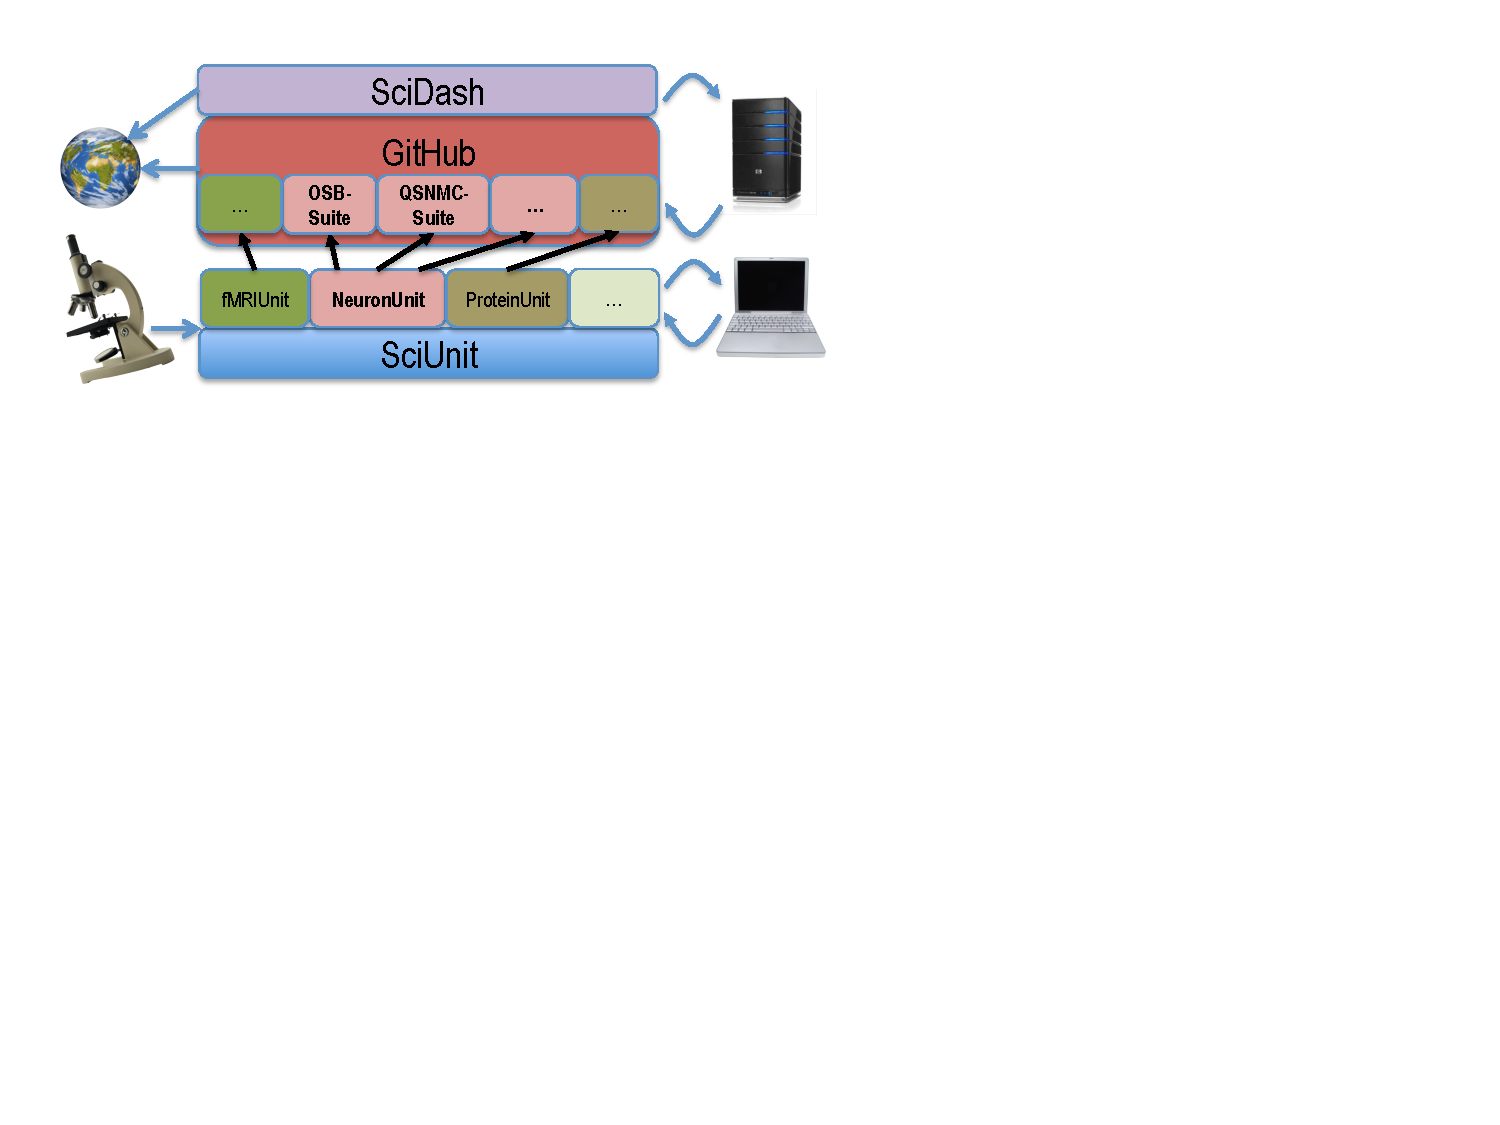
\includegraphics[scale=0.65]{sciunit_overview.pdf}
\caption{Proposal overview. \scriptsize{i) The \textit{SciUnit} framework can generate discipline-specific libraries of tests and model interfaces.  \textit{NeuronUnit} is proposed and described here.  Experimental data guides test development; model generation informs and is informed by the collections in a \textit{SciUnit} library.  Each \text{SciUnit} library on GitHub is indexed by the \textit{SciDash} web application.  \textit{SciDash} automatically runs the test collections in each library and publicly displays the results.}}
\vspace{-10px}
\label{fig:sciunit_overview}
\end{wrapfigure}
\leavevmode

Our framework is organized around simple executable \emph{validation tests} that compute agreement between a model prediction and an experimental observation. Model \textit{scope} is identified with the set of tests that a model is capable of taking and \textit{validity} is identified with how well the model performs on these tests.

This methodology is inspired by the ubiquitous practice of \emph{unit testing} in software engineering. A \emph{unit test} evaluates whether a portion of a computer program (often a single function) meets one simple correctness criterion. A \textit{suite} of such tests \emph{covering} the range of desired program behaviors helps validate the functionality of the program overall. Due to the narrow scope of each test, failed tests help precisely identify which parts of a program are functioning incorrectly. Developers often write unit tests before writing the program itself, following a methodology called test-driven development (TDD)\cite{beck2003}. When written early, tests serve as a partial program specification, guiding development and allowing developers to measure progress simply by looking at the proportion of tests passing at any point during development. When modifications are made, developers can ensure that \emph{regressions} have not appeared by checking that all tests which passed before a change continue to pass afterwards. The success of unit testing and TDD in practice suggests that validation testing may be a practical foundation for model validation as well.

Inspired by these ideas, we propose here the development of \textbf{\textit{SciUnit}}, a framework for validation testing; \textbf{\textit{SciDash}}, a web application for collaboratively developing and discovering test suites, visualizing test results and organizing test-based competitions; and \textbf{\textit{NeuronUnit}}, a repository of tests and associated utilities for single-neuron neurophysiology that will serve as the most substantial initial case study for our tools.

\subsection{\textit{SciUnit}: A Simple Validation Testing Framework}
Conceptual and practical simplicity -- the absence of ``heavy-lifting'' -- is an essential requirement for community participation. Our design does not require the release of raw data or storage in standard formats. Instead, salient aspects of the data are abstracted away behind a test definition. Similarly, implementation details of a model (e.g. its programming language) need not be public or standardized -- the implementation must simply be wrapped to expose a standardized interface, so that tests can access model capabilities. Each community can collaboratively specify model interfaces capturing high-level operations of their preferred modeling formalisms. Existing modeling standards (e.g. NeuroML\cite{neuroml_url,gleeson_neuroml:_2010}) are leveraged to simplify this process. \textbf{Thus, the first product of this proposal is an object-oriented validation testing framework called \textit{SciUnit}, written in Python, that makes test construction (from data) and test-driven model execution easy and flexible.} 

\begin{figure}
\small
\begin{python}
class SpikeCountTest(sciunit.Test):
  """Tests a model that generates spike counts from currents.

  parameters:
    inputs: list of input currents traces (in nA) as numpy arrays
    means, stds: list of observed means and standard deviations of 
      spike count distribution in response to corresponding input
  """
  def __init__(self, inputs, means, stds):
    self.inputs, self.means, self.stds = inputs, means, stds
	
  required_capabilities = [SpikeCountFromCurrent]
	
  def run_test(self, model):
    inputs, means, stds = self.inputs, self.means, self.stds
    n = len(inputs)
    counts = numpy.empty((n,))
    for i in xrange(n):
      counts[i] = model.spike_count_from_current(inputs[i])
      
    # TODO how does the QSNMC measure goodness-of-fit?
    return sciunit.AveragePValue(result, related_data={
      "inputs": input_current,
      "obs_means": means,
      "obs_stds": stds
    })
\end{python}
\vspace{-5px}
\caption{A single neuron spike count test family implemented in \textit{SciUnit}}
\label{fig:rate_test}
\vspace{-10px}
\end{figure}
%\leavevmode
\subsection{Example: Neural Membrane Potential Dynamics} To make our proposal concrete, we describe a test suite related to neurophysiology. These tests are derived from experiments where stimuli were delivered to neurons of a particular type, as somatically injected current (in pA), while the somatic membrane potential of each stimulated cell (in mV) was recorded and stored.  A model claiming to capture the this cell type's membrane potential dynamics must be validated in several ways. 

One simple validation test would check for correspondence between the distribution of the number of action potentials produced by the model (called a \emph{spike count}) and the distribution observed in the data, in response to the same stimulus. This test would ask a candidate model to produce a predicted spike count for each stimulus and then check whether the prediction was consistent with the empirically-observed spike count distribution in response to the same stimulus.  The test creator would specify the metric for success; for example, a model that, for each stimulus, produced a spike count falling in the 95\% confidence interval of the empirical data distribution might pass this example test\todo{the QSNMC used a chi-squared metric, we should probably use that too}. 

A number of other tests would be included to complete the suite. For example, the QSNMC defined 17 other validation criteria for this sort of data, based on measures like spike latencies (SL), mean subthreshold voltage (SV), interspike intervals (ISI) and interspike minima (ISM) that can be extracted from the data\cite{jolivet_quantitative_2008}. They then defined a combined metric favoring models that broadly succeeded at meeting these individual criteria, to produce an overall ranking. Such combined criteria are simply validation tests that invoke other tests to produce a result.

Importantly, the validation criteria are made explicit by the specification of a test suite, so modelers need not guess which criteria are being used to validate or invalidate their model. Validation criteria are subject to debate (indeed, the QSNMC criteria changed between 2007 and 2008 due to such debates), and scientists who wish to promote different criteria need only derive alternative test suites. In many cases, models require no modifications to take the new tests because the same type of data is being requested.

\subsection{Validation Testing with \emph{SciUnit}} 
The first product of this proposal is a simple validation testing framework to support building test suites like the one described above. This framework, called \emph{SciUnit}, is written in Python and uses Python's object-oriented facilities to simplify test construction (from data) and execution\cite{python_oo_url}.  It also requires the Numpy numerics library common to most Python scientific computing projects\cite{numpy_url}.

Fig. \ref{fig:rate_test} shows how a scientist would implement the spike count test described in the preceding section with \textit{SciUnit}. A \textit{SciUnit} validation test is an {instance} of a Python class implementing the \verbx{sciunit.Test} interface. Here, we show a class \verbx{SpikeCountTest} taking three \emph{parameters} in its constructor (in Python, the constructor is always named \verbx{__init__}), described in the documentation string (lines 2-7). To create a \emph{particular} spike count test, we instantiate this class with particular experimental observations. For example, given observations from hippocampal CA1 cells, we can create a test as follows:
\begin{python}
  CA1_sc_test = SpikeCountTest(CA1_inputs, CA1_means, CA1_stds)
\end{python}

We emphasize a crucial distinction between the \textit{class} \verbx{SpikeCountTest}, which can be thought of as representing a \emph{parameterized family} of validation tests, and the particular \textit{instance} \verbx{CA1_sc_test}, which is an individual validation test. Parameterized test families package common testing logic that can be reused to instantiate tests based on new data without having to rewrite the testing logic. As we describe below, we expect communities to build repositories of such families so that test generation will often consist simply of instantiating an existing family with particular experimental parameters and data. For single-neuron tests, we refer to this repository as \textit{NeuronUnit} (Sec. \ref{sec:neuronunit}). 

% Testing in SciUnit proceeds in three phases (Figure 1):\todo{this spacing seems unnecessarily small}
%\begin{enumerate}
%\item Capability Checking: The test checks to see that the model is capable of taking the test; i.e., that it exposes the needed functionality for the execution phase to proceed.
%\item Test Execution: The model is executed to produce the model output by interacting with its supported capabilities.  If the model is described according to a standard specification, e.g. NeuroML, this corresponds to loading it into a supported simulator and executing it. 
%\item Output Validation: The model output is compared to empirical data to determine whether the model passes.  This comparison can be of several types: for deterministic models, we may extract a matching quantile from a data distribution; for stochastic models, we may compute a measure of agreement between model output and data distributions, e.g. the Kolmogorov-Smirnov statistic.  Validation is ultimately pass/fail, but in some cases the result generated in this phase also includes a continuous statistic so that models can be ranked based on their test results in a more fine-grained manner.   
%\end{enumerate}
%\todo{Fix figure reference}
%
\begin{figure}
\begin{python}
class SpikeCountFromCurrent(sciunit.Capability):
  def spike_count_from_current(self, input): 
    """Takes a numpy array containing current stimulus (in nA) and
    produces an integer spike count. Can be called multiple times."""
    raise NotImplementedError("Model does not implement capability.")
\end{python}
%\vspace{-15px}
\caption{An example capability specifying a single required method.}
\label{fig:capability}
\end{figure}

\begin{figure}
\begin{python}
class TrainSpikeCountFromCurrent(sciunit.Capability)
  def train_with_currents(self, currents, counts):
    """Takes a list of numpy arrays containing current stimulus (in nA) and
    observed spike counts. Called once."""
    raise NotImplementedError("Model does not implement capability.")
\end{python}
%\vspace{-15px}
\caption{Another capability specifying a training protocol (not used by the test in Figure \ref{fig:rate_test}).}
\label{fig:training}
\end{figure}

Classes that implement the \verbx{sciunit.Test} interface must contain a \verbx{run_test} method that receives a candidate model as input and produces a \textit{score} as output. Models are instances of \verbx{sciunit.Model} and scores are instances of \verbx{sciunit.Score}. To specify the interface between the test and the models within its scope, the test author provides a list of \emph{capabilities} in the \verbx{required_capabilities} attribute, seen on line 5 of Fig. \ref{fig:rate_test}. Capabilities are analogous to \emph{interfaces} in languages like Java. In Python, they correspond to classes with unimplemented members. In \textit{SciUnit}, we require that such classes be tagged as capabilities by inheriting from \verbx{sciunit.Capability} to allow them to be discovered by our infrastructure (discussed below). The example capability used in Fig. \ref{fig:rate_test} is shown in Fig. \ref{fig:capability}. A simple \emph{model family} implementing this capability is seen in Fig. \ref{fig:simple_model} which simply produces a spike count by applying a linear transformation to the mean of the input current. The model family is parameterized by the scale factor and offset. To create a particular model, a modeler must choose particular parameters and instantiate the class, just as with tests:
\begin{python}
CA1_linear_model_heuristic = LinearModel(3.0, 1.0)
\end{python}
Here, the parameters to the model are picked by the modeler heuristically or based on externally available training data. An alternative test design would be to specify a second capability (Fig. \ref{fig:training}) and modify the test to provide training data, thereby requiring that the model be able to adapt its parameters without human feedback. Whether to build training into the test protocol is a choice left to each modeler. Fig. \ref{fig:rate_test} does not include a training phase, but if external training data is available, models that implement the training capability (i.e. implement its methods) can be trained explicitly by calling the capability method just like any other Python method:
\begin{python}
CA1_linear_model_fit = LinearModel()
CA1_linear_model_fit.train_with_currents(CA1_training_in, CA1_training_out)
\end{python}
\begin{figure}
\begin{python}
class LinearModel(sciunit.Model, SpikeCountFromCurrent, 
    TrainSpikeCountFromCurrent):
  def __init__(self, scale=None, offset=None): 
    self.scale, self.baseline = scale, offset
    
  def spike_count_from_current(self, input):
    return int(self.scale*numpy.mean(input) + self.offset)

  def train_with_currents(self, currents, counts):
    means = [numpy.mean(c) for c in currents]
    [self.scale, self.offset] = numpy.polyfit(means, counts, deg=1)    
\end{python}
\caption{A simple model that returns a spike count by scaling the mean of the input by a fixed parameter.}
\label{fig:simple_model}
\end{figure}
In the test in Fig. \ref{fig:rate_test}, the \verbx{run_test} method simply calls the \verbx{spike_count_from_current} capability method  to produce spike count predictions for each input current on line 18. The resulting spike count is compared to the empirical mean and standard deviation on ...\todo{need to figure this out} to produce a mean p-value. In addition to the score itself, the returned score object also contains metadata that can be used to examine the result in detail. In this test we saved the inputs and observed means and standard deviations alongside the score by using the \verbx{related_data} parameter. We discuss visualization of results in Sec. \ref{sec:scidash_activities}.

Finally, a test is executed against a model instance, using the \verbx{sciunit.run} function:
\begin{python}
score = sciunit.run(CA1_sc_test, CA1_linear_model_heuristic)
\end{python}

The \verbx{sciunit.run} function operates in three phases: \textbf{(1) Capability Checking}: The model is verified as capable of taking the test by checking each capability in the test's \verbx{required_capabilities} attribute; \textbf{(2) Test Execution}: The test's \verbx{run_test} method is called to execute the model and cache its output. \textbf{(3) Output Validation}: \verbx{run_test} returns an instance of a \verbx{sciunit.Score} subclass containing a goodness-of-fit metric between the model output and the data used to instantiate the test.  Any errors that occur during this process are reported by raising an appropriate exception.

\subsection{\textit{SciUnit} Test Suites}
A test suite is a collection of tests designed to validate a model against several mutually coherent requirements, i.e. various summaries of the data.  The following is a test suite that could be used for the QSNMC.  
\begin{python}
CA1_suite = sciunit.TestSuite([CA1_sc_test, CA1_sl_test, CA1_sv_test, CA1_isi_test, CA1_ism_test])
\end{python}
When a test suite is executed against a model, it produces summary data that can be shown on the console or visualized by other tools, such as the web application described in the Sec. \ref{sec:scidash}.

\begin{table}[h]\footnotesize
\caption{Glossary of Terms}
\label{table:glossary}
\begin{tabular}{| c | p{13cm} |}
\hline
Data & The measurements yielded by an experiment.\\ \hline  
Model & An executable function that aims to explain, reproduce, or predict experimental data.  More generally, a candidate.\\ \hline
Model Family & A class that generates a set of related model instances. Each model instance from one family differs according to the set of parameters (corresponding to a particular experimental design, or set of training data) with which it was initialized.\\ \hline  
Validation	 & The process of assessing the agreement between model output and experimental data.\\ \hline
(Validation) Test & A function that executes a model and scores the model’s output against a summary of experimental data. One experiment can inform the development of many tests.\\ \hline  
Test Family & A class that generates a set of related test instances.  Test instances from within one family differ only quantitatively, according to the data used to initialize them.  All tests from one family attempt to validate the same property of a model.\\ \hline
Test Suite & A collection of tests, each of which attempts to validate a different property of a model.\\ \hline  
Score & A value summarizing the performance of a model on a test. This can be a measure of the goodness of fit between model output and experimental data.\\ \hline
Scope & A list of tests that a model is eligible to take, indicating the range of experimental data that the model might be able to explain or replicate.\\ \hline
Capability & 	A contract that states that a model is able to produce results of a particular form. For example, a Hodgkin-Huxley neuron model is capable of producing a membrane potential time-series, whereas a model without a notion of voltage is not.\\ \hline
Record & An indication of the test score achieved by a model, along with any initialization conditions.\\ \hline
Record Suite & A list of records associated with a model.  This summarizes the scope and validity of the model.\\ \hline  
\end{tabular}
\end{table}

\subsection{Community Workflow}
In software engineering, unit tests are produced by a program's community of developers. Correspondingly, a scientific community's members can collaboratively produce suites of validation tests in common source code repositories. Each test specifies the model requirements, and provides a procedure for determining whether a candidate model (the input to the test) is consistent with a particular summary of experimental observations (the parameters of the test). Model performance on a collaboratively curated suite of validation tests can serve as justification of claims regarding the model's validity as a description of the scientific system characterized by the test suite.
This workflow continuously produces a summary of the field, indicating which models are capable of taking each test, i.e. whether the test falls within the model's scope; and for each capable model, how well it performed, i.e. its validity.  Model usefulness becomes a function of the weight given to each test, determined per investigator or by community consensus. This test-driven scientific workflow leverages the desire of modelers to promote their models' virtues -- test suites represent clear \emph{challenges}, issued by experimentalists to the community, and passed tests certify success for the modelers. As more data is gathered and test suites are refined, past models can be tested continuously againt current empirical knowledge in a fully-automated manner, because the interface between tests and models is fixed.  

\subsection{\textit{SciDash}: A Community web application}\label{sec:scidash}
This framework is most effective when the current state of a research area is represented by a collection of tests and models. This requires coordination among research groups, so community-oriented cyberinfrastructure to support test suite creation and summarization, building upon \textit{SciUnit}, is essential.
We propose a service, called \textit{SciDash}, utilizing existing infrastructure for coordinated development of software repositories, focusing on GitHub\cite{github_url}\cite{ram_git_2013}. A suite of related tests will be contained in a GitHub repository with a stereotyped high-level structure that allows the \textit{SciDash} web application to discover, index and summarize it on an ongoing basis (Fig. \ref{fig:scidash_repo}).
The portal, a web application written using the pythonic Django framework\cite{django_url} will serve as a central location where scientists can discover relevant test suites, determine test requirements, and summarize the results of test execution on submitted models. Test results can be visualized as a ``record matrix'' composed of large numbers of model/test combinations (Table \ref{table:record_matrix}, discussed in section~\ref{sec:education}, provides a toy example).  Each row in this matrix will contain results for all tests taken by one model and would serve as clear evidence of that model's scope and validity.  Models, tests, and records will be stored on GitHub, pointed to by hyperlinks in the record matrix. \textit{SciDash} will serve as a public record of competition among models, facilitating and encouraging data-driven development among modelers.
\textbf{Thus, the second product of this proposal is a web application called \textit{SciDash}, whose back-end can index test suite repositories collaboratively developed on GitHub, and whose front-end offers users a simple environment for discovery and evaluation of models, tests, and results.}  

\subsection{\textit{NeuronUnit}: A Suite of Tests for Neurophysiology}\label{sec:neuronunit}
To demonstrate the utility of these tools, an initial case study must be conducted. Because we have substantial experimental and computational neurophysiology training and expertise, we target this domain. By using machine-readable models from the Open Source Brain repository, and corresponding machine-readable data from resources like The NeuroElectro Project\cite{neuroelectro_url}, our efforts will produce a body of useful tests that also serve as a demonstration of the test-driven workflow that other areas in the biological sciences can leverage.  \textbf{The third product of this proposal is \textit{NeuronUnit}, a large suite of data-driven tests and model interfaces for a representative set of canonical neurophysiology models, all publicly available. A case study examining the implementation of \textit{NeuronUnit} will inform development of domain-specific test suites in other biology sub-fields.}

% Section 3.
\section{Preliminary Activities}

\subsection{\textit{SciUnit} Activities} We have developed most of the core testing framework, \textit{SciUnit}, under a free, open-source license at the project development repository\cite{sciunit_url}.  We implemented it using the Python programming language\cite{python_url} due to its widespread adoption across the quantitative sciences. Python also supports interoperability with other major languages used within science, including C, R\cite{r_url}, and MATLAB\cite{matlab_url}. The functionality we have described could also be readily translated into any programming language with comparable facilities.  Table \ref{table:glossary} provides definitions of terms.  

\begin{figure}
\begin{python}
class CA1PyramidalCellModel(NeuroConstructModel,
				            capabilities.ReceivesCurrent):
	"""CA1 Pyramidal Cell model from /neuroConstruct/osb/hippocampus/
	CA1_pyramidal_neuron/CA1PyramidalCell"""
	def __init__(self,**kwargs):
		# Put any other initialization here.
		project_path = os.path.join(candidates.putils.OSB_MODELS,
									"hippocampus",
									"CA1_pyramidal_neuron",
									"CA1PyramidalCell",
									"neuroConstruct")
		candidates.NeuroConstructModel.__init__(self,project_path,**kwargs)
		super(CA1PyramidalCellModel,self).__init__(**kwargs)
\end{python}
%\vspace{-15px}
\caption{A candidate class corresponding to a CA1 Pyramidal Cell model from Open Source Brain}
\label{fig:ca1_model}
\end{figure}

\begin{wrapfigure}[18]{r}{0.5\textwidth}
%\centering
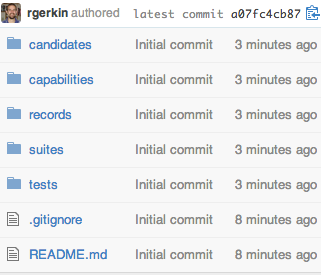
\includegraphics[scale=0.7]{scidash_github.png}
\caption{A \textit{SciDash} repository on GitHub}
\label{fig:scidash_repo}
\end{wrapfigure}
\leavevmode
\todo{Update this figure when SciDash repo structure is finalized} 
\subsection{\textit{SciDash} Activities}\label{sec:scidash_activities}
We have also begun work on the \textit{SciDash} web application, which point to test suite repositories and aggregates test results for scientific communities. A development version written using Django (a Python web framework) is currently live\cite{scidash_url}.  It is populated with models and tests from the educational illustration in Table \ref{table:record_matrix} (section~\ref{sec:education}).  We have implemented \textit{SciDash} in three layers.  The \textbf{first layer} is completely in the control of individual developer communities, and consists of git repositories.  Git is the most popular implementation of ``version control'' among developers today\cite{ram_git_2013}, and is increasingly used for open science projects (e.g. OSB\cite{osb_url}).  The GitHub website\cite{github_url} is the most popular location for collaboration of code development using git.  It organizes millions of git repositories, provides numerous tools for collaboration and discussion, and easy-to-use GUIs for every operating system.  Git and GitHub also meet all the requirements of a means for collaboration on test suite repositories: they are open (but provide user access controls), the entire history of code changes is visible; and collaboration is simple.  For example, anyone can ``fork'' a repository on GitHub, make desired changes, and optionally submit those changes back to the main repository for inclusion.  These virtues make GitHub an ideal first layer for \textit{SciDash}.  We created a vanilla test suite repository\cite{scidash_repo_url} on \text{SciDash} (Fig. \ref{fig:scidash_repo}).  We are currently developing an API for \textit{SciDash} to identify all similarly structured repositories (by tracking the lineage of the repository above using the GitHub API).  This list of repositories will be indexed by \textit{SciDash} to form the \textbf{second layer}, an overview of the state of all \textit{SciDash} repositories on GitHub.  This index will be searchable and filterable on the \textit{SciDash} website to identify repositories of interest to a particular research community.  The \textbf{third layer} will be a ``dashboard'' view of the state of a field, visible through a matrix of records for model/test combinations in a GitHub repository (Fig. \ref{fig:scidash_repo}.  Each record will link to the tests results (stored in the repository), displaying line-by-line the executed code and intermediate output statements, as well as the underlying models and tests.   

\subsection{\textit{NeuronUnit} Activities}
\label{sec:neuronunit_acitivities}
Here we describe standard neuroinformatics tools we have adopted to develop \textit{NeuronUnit}\cite{neurounit_url}.  

\subsubsection{Candidates from NeuroML Models}\label{sec:neuroml_candidates}
NeuroML is a standardized model description language for neuroscience\cite{gleeson_neuroml:_2010}. It permits many neurophysiological/neuroanatomical models to be described in a simulator-independent fashion, and executed across many popular simulators due to inter-conversion capabilities of the NeuroML API.  Because NeuroML is an XML specification, model descriptions can be validated for correctness and queried for model properties and components, exposing potential capabilities.  It is ideal for model sharing, curation, and for answering both \textit{what} and \textit{how} programatically.  

NeuroConstruct\cite{neuroconstruct_url,gleeson_neuroconstruct:_2007} is a simulation manager that takes NeuroML models and hands off simulation to supported neural simulators. To this end, \textit{NeuronUnit} offers a \verbx{sciunit.Candidate} subclass called \verbx{NeuroConstructModel}, instantiated with the path to a NeuroML model.  Because NeuroML can describe such a wide range of models, \verbx{NeuroConstructModel} makes few assumptions about them: that they each is \verbx{TimeIntegrable}, and \verbx{HasMembranePotential}.  It is subclassed to test \textit{specific} NeuroML models (Fig. \ref{fig:ca1_model}). 

The Open Source Brain project (OSB,\cite{osb_url}) curates many models described in NeuroML. OSB-curated projects are converted from their native format into NeuroML, and run on major neural simulators\cite{neuron_url,genesis_url,nest_url,moose_url}. Concordance between model output (beginning with the NeuroML description) and reference output (from native simulator source files) is reported for each model.  Thus, OSB is an excellent source of models that, in addition to being open source, are sufficiently described to enable validation.   The hippocampal CA1 pyramidal cell is commonly modeled, and we implement one such model hosted on OSB\cite{osb_ca1_url} by simply declaring a \verbx{CA1PyramidalCellModel} class , deriving from \verbx{NeuroConstructModel}.  This basic implementation simply ``wraps'' the functionality of the existing model, and only the code shown in Fig. \ref{fig:ca1_model} is required.  All OSB models, and indeed any NeuroML model, can be tested similarly.  Working together with OSB is part of our \textbf{first collaboration}, and our integration efforts can be publicly tracked\cite{neuroconstruct_rgerkin_url}.  

Spanning a range of scales and original development environments, all OSB models are formally described using NeuroML, as are all model components and sub-components, such as cells, ion channels, calcium stores, etc.  These models are regularly executed on OSB servers to ensure that their output remains consistent as they are updated.  Therefore, OSB can confirm that they \textit{do} work, while linked journal articles, on-site wiki, and code inspection can establish \textit{how} they work. However, there is no mechanism for establishing \textit{how well} they work, i.e. how well the models accord with data.  \textit{SciUnit} fills this gap by helping OSB (and the larger biology community) assess models using data-driven tests in the \textit{NeuronUnit} library.  \textit{SciUnit} can be applied similarly to other biology sub-disciplines using \textit{NeuronUnit} analogues written by the corresponding communities.    

\subsubsection{Capabilities from NeuroTools}
NeuroTools\cite{neuralensemble_url} is a Python library supporting tasks associated with analysis of neural data (or model output), such as membrane potential time series, spike trains, etc. It is an open source and actively developed project, containing reliable algoithms on which to base neurophysiology tests.

We use NeuroTools to implement \textit{SciUnit} capabilities in \textit{NeuronUnit} (Fig. \ref{fig:NeuronUnit_example}).  For example, a NeuroTools \verbx{AnalogSignal} object (e.g. a membrane potential time series) has a threshold detection method that returns a NeuroTools \verbx{SpikeTrain} object.  A \textit{NeuronUnit} \verbx{HasSpikeTrain} Capability requires that  \verbx{getSpikeTrain} method be implemented.  \verbx{NeuroConstructModel} does so by placing \verbx{AnalogSignal.threshold_detection} inside \verbx{getSpikeTrain}.  Many such NeuroTools objects are similarly exchanged between \verbx{NeuroConstructModel} methods.  This simplifies test writing, since basic model output properties are obtained trivially using NeuroTools object methods, and these NeuroTools objects are easily extracted from model output using candidate models subclassing \verbx{NeuroConstructModel}.  

\subsubsection{Reference Data for Tests from NeuroElectro}
Answering \textit{how well} requires validation testing against data. The NeuroElectro project\cite{neuroelectro_url} is an effort to curate all published single cell neurophysiology data\cite{tripathy_neuroelectro:_2012}.  Currently, up to 27 electrophysiological properties are reported for 93 cell types, spanning $>$ 2000 single pieces of published data extracted from article tables.  \textit{NeuronUnit} tests are easily constructed using the NeuroElectro API for reference data. Tests can be based upon data from single journal articles, or from ensembles of articles with a common theme (e.g. about a particular neuron type).  The former is illustrated in Figure \ref{fig:NeuronUnit_example}.  Associated statistics of that data (e.g mean, standard error, and sample size) are attached and enable judgement of model output according to a chosen scoring mechanism.\todo{Should there actually be an example of workflow with NeuroElectro here?} While NeuroElectro alone cannot judge all model aspects, it can serve to validate basic features of many models, such as resting membrane potential, action potential width, after-hyperpolarization amplitude, etc.  As NeuroElectro is the only publicly curated source of such data, it represents a key component for \textit{NeuronUnit} test constuction.  Continued development of the NeuroElectro API, through which data are systematically exposed to test authors, represents our \textbf{second collaboration}\cite{neuroelectro_dev_url}.  

\begin{figure}
\label{fig:ca1_model}
\begin{python}
class CA1PyramidalCellModel(NeuroConstructModel,
				            capabilities.ReceivesCurrent):
	"""CA1 Pyramidal Cell model from /neuroConstruct/osb/hippocampus/
	CA1_pyramidal_neuron/CA1PyramidalCell"""
	def __init__(self,**kwargs):
		# Put any other initialization here.
		project_path = os.path.join(candidates.putils.OSB_MODELS,
									"hippocampus",
									"CA1_pyramidal_neuron",
									"CA1PyramidalCell",
									"neuroConstruct")
		candidates.NeuroConstructModel.__init__(self,project_path,**kwargs)
		super(CA1PyramidalCellModel,self).__init__(**kwargs)
\end{python}
\vspace{-5px}
\caption{A candidate class corresponding to a CA1 Pyramidal Cell model from Open Source Brain}
\vspace{-10px}
\end{figure}
%\leavevmode

% Josh: In particular I'd like to
%see more discussion of the overview SciDash will give of the test
%results. Are all tests equal? What aggregation functions will you
%provide?How will a new user (or journalist as you suggest in one of
%the concluding sections) be able to reasonably quickly understand "how
%well" a model predicts the data?

% Section 4.
\section{Research and Development Plan}
In order to make immediate use of \textit{SciUnit} and populate \textit{SciDash} with models and tests, we will initially focus on \textit{NeuronUnit} development, to serve one discipline (neurophysiology) without compromising generalizability. This will enable rapid feedback from a familiar experimental community, guiding development.  

\subsection{A Complete Pipeline}
Although the tools described in Sec. \ref{label:neuronunit_acitivities} do not exhaust the possible sources of models, capabilities, and test data, they provide an immediate point of entry into the neurophysiology community and powerful demonstration of our proposal.  In the \textit{NeuronUnit} repository\cite{neurounit_url} is a runnable script (\textit{examples.py}) demonstrating a complete testing pipeline.  It (1) selects an OSB model; (2) simulates it using NeuroConstruct; (3) tests the widths of the resulting action potentials, extracted and computed using NeuroTools, against NeuroElectro data downloaded on-the-fly, using a \textit{NeuronUnit} test class called \verbx{SpikeWidthTest}; and (4) computes and prints a test score.\ref{fig:neuronunit_example}

\begin{figure}
\begin{python}
# Get reference data for spike width of CA1 Pyramidal cells from neuroelectro.org. 
reference_data = NeuroElectroSummary(neuron={'id':85}, ephysprop={'id':23})
reference_data.get_values()  # Get and summary data for the above. 
candidate = CA1PyramidalCellModel(population_name="CG_CML_0") # Initialize the model with some parameters.
test = SpikeWidthTestDynamic( # Initialize the test.    
	reference_data = {'mean':reference_data.mean, 'std':reference_data.std}, # Summary statistics from the reference data
	candidate_args = {'current':40.0}, # Somatic current injection in pA.  
	comparator = ZComparator), # A comparison class that implements a Z-score.  
result = sciunit.judge(test,candidate) # (1) Check capabilities, (2) take the test, (3) generate a score and validate it, (4) bind the score to candidate/test combination. 
result.summarize() # Summarize the result.  
\end{python}
\caption{Working example of a NeuronUnit testing}
\label{fig:neuronunit_example}
\end{figure}

\subsection{Creating New Candidates, Capabilities and Tests}
\textit{NeuronUnit} provides base classes to enable rapid generation of candidates, capabilities, and tests for neurophysiology data.  However these objects can also be created from scratch, requiring only adherence to the core \textit{SciUnit} interface.  For example, a Candidate could implement an \verbx{integrate} capability method by wrapping execution of a MATLAB script and a \verbx{get_spikes} capability method by parsing a .csv file on disk; and a test could be initialized using empirical spike rates collected in the lab.  While this is not meet the idealized vision of model development and testing, in practice this is likely to be a common scenario.  As part of our outreach efforts (Sec. \ref{sec:broader_impacts}) we plan to train modelers in the use of this framework, and we will encourage them to use it as part of the workflow of their choice.  Adoption in traditional, custom workflows would be reflected in the Methods sections of articles.  

\subsection{\textit{SciDash} Implementation}
\textit{SciDash} will point to collections of models and tests as they become available, and display corresponding test results.  This will provide a dedicated resource for evaluating model validity, and the progress of the initiative, including community adoption, will be transparent from the number and size of the repositories indexed.  The source code is being developed openly\cite{scidash_portal_repo_url}, supporting organizations that want their own private dashboard for models or datasets not yet ready for release.  Such organizations can set their own root \textit{SciDash} repository, indexing only those repositories forked from that root.  

There are many possibility for visualization of specific test results though \textit{SciDash}.  When a test record is selected from the record matrix (Table \ref{table:record_matrix}, section~\ref{sec:education}), it can point to a Sage notebook\cite{sagenb_url}, whose ``worksheets'' facilitate visualization and storage of executed code.  While Sage was written for Python, the notebook also supports the execution of code and visualization of outputs from other programming languages, making possible worksheets based on MATLAB, Mathematica, and other popular environments for modeling.  Even with \textit{SciUnit} written in Python, calls to other languages can still be issued, and their results visualized using these worksheets.

Community-moderated comments on GitHub will allow test-makers and test-takers to discuss issues associated with test suites.  On GitHub, these takes the form of ``issues,'' commit messages, and comments surrounding merge requests from forked repositories.  Thus, disagreements about the appropriateness of a test can be openly aired and in many cases resolved.  The \textit{SciDash} website itself can also support public comment to extend the features of GitHub.  More importantly, we will enable sorting and filtering of \textit{SciDash} results by repository statistics, e.g. the volume of activity and the number of followers, via the GitHub API.  This will allow the most important test suites, as judged by each community, t be featured prominently on \textit{SciDash}.  Simple tagging should enable filtering by subject matter.  We also will support open authentication via existing web applications (Google, Yahoo, Twitter, etc.), lowering the barrier to participation.  The \textit{SciDash} backend will consist of a MySQL relational database, updated regularly using the GitHub API to populate record matrices.  

\textit{SciDash} will reguarly run scripts that (1) read the GitHub repositories, (2) run any outstanding tests on new or existing models, and (3) format the results.  In order to quickly populate \textit{SciDash} with repositories that are both useful and illustrative, we will use \textit{SciUnit} to recapitulate the results of some ``settled'' competitions as \textit{SciDash} repositories, i.e. we will encode the competition rules as tests and \textit{SciDash} will then index the results.  There are several examples of settled competitions which have publicly available rules, entries, and results against which to check\cite{jolivet_quantitative_2008}.  

\subsection{Measuring Progress}
We will follow this example and increase the number of \textit{NeuroConstruct} capabilities implemented until adequate coverage of models on OSB is achieved.  Progress will be tracked in an OSB \textit{SciDash} repository.  One measure of success will be construction of tests that parallel journal-published figures associated with OSB models.  However, this will represent only a small subset of all possible model/test combinations.  Another measure of success will be the nimber of commits, contributors, and forks (on GitHub) for this repository, which are viewable on all GitHub repository pages.  An even more concrete measure of success would be for competitions to be run using \textit{SciUnit}, with outcomes tracked on \textit{SciDash}.   To this end we will arrange to run the next QSNMC using \textit{NeuronUnit}.  

\subsection{Project Milestones}
\begin{description}
\item[Year 1:] a) Refine the \textit{SciUnit} core and complete the corresponding Python module; b) implement \textit{NeuronUnit} tests using NeuroElectro data and capabilities using NeuroTools functions; c) Submit a manuscript describing the idea and tools.  
\item[Year 2:] a) Automatie OSB model testing, greatly increasing the number and scope of models tested; b) Continue to define \textit{SciUnit} model capabilities via collaborative development of NeuroTools; c) Aggregate new community-provided datasets to generate \textit{NeuronUnit} tests; d) Populate \textit{SciDash} with a dozen repositories corresponding to focused model and test collections.    
\item[Year 3:] a) Fully document \textit{SciUnit} and associated tools to encourage adoption; b) Continue to write tests and specify (existing, published) models in NeuroML for testing; c) Submit a manuscript describing the overall results and promoting \textit{SciDash}; d) Submit a manuscript describing the array of usable tests and tools in \textit{NeuronUnit}; e) Promote use of these tools at conferences and workshops, generating community interest and inspiring development of \textit{NeuronUnit} analogues in other biology disciplines.  
\end{description}

\subsection{Challenges}
Here we describe theoretical and practical challenges to implementation, and how they can be overcome.

\subsubsection{Participation from Modeling Communities}
Modelers may not want to expose model capabilities, a requirement of test-taking.  We anticipate four solutions: \textbf{First}, interfacing a model to \textit{SciUnit} requires only implementing selected model capabilities.  Often this means identifying native model procedures that satisfy a capability, and wrapping their functionality.  This can require as little as one line of code.  Importantly, the modeler is not required to expose or rewrite any model flow control.  \textbf{Second}, we support multiple environments automatically by using NeuroML\cite{gleeson_neuroml:_2010}, and other simulator-independent model descriptions are possible for other domains. Automated generation of NeuroML from native model source code is in development (Gleeson, personal communication); for the popular NEURON simulator, this functionality is already mature and in use.  This minimizes modeler effort for a large and growing number of models.  \textbf{Third}, modelers have an incentive to demonstrate publicly their models' validity.  Participation in public modeling competitions (Sec. \ref{sec:existing_efforts}) illustrates this incentive.  \textbf{Fourth}, modelers have an incentive to use \textit{SciUnit} during development (see TDD, above) to ensure that ongoing development preserves correspondence between model and data.  A popular test suite can represent a ``gold standard'' by which progress during development is judged.

\subsubsection{Participation from Experimental Communities}
Experimentalists may not want to write tests derived from their data.  We anticipate four solutions: \textbf{First}, tests require no special data formatting, only a list of required  capabilities (for selecting eligible models), optional metadata (as run-time arguments), and statistical data summary (for scoring tests) are required.  A unit test is focused, and does not require arbitrary computations on data.  For example, suppose intracellular current injection evokes 100 action potentials, the width of which is of interest.  Writing the test consists of selecting ReceivesCurrent and ProducesActionPotentialShape capabilities (one line of code each), computing the mean and variance of action potential widths (one line of code), specifying current injection parameters, e.g. amplitude and duration (two lines of code), and selecting a scoring mechanism from \verbx{sciunit.scores}, e.g. (colloquially) ``Must be $<$ 1 standard deviation of the mean'' (one line of code).  This example can be found in \verbx{NeuronUnit.tests.SpikeWidthTest}; heavy-lifting is done by the interface. \textbf{Second}, data-sharing is becoming accepted, test-writing can be distributed across scientists, including non-experimentalists with other aims. \textbf{Third}, many tests can be automatically generated using the NeuroElectro API, and the continued emergence of such data-aggregation initiatives will expand these possibilities. \textbf{Fourth}, an incentive to write tests for one's data exists: the ability to identify the models that give the data clear context and impact. 

\subsubsection{Diversity of Levels and Kinds of Models and Data}
The diversity of topics in biology is vast. \textbf{First}, we address this by providing an interface allowing modelers to express specific capabilities.  This capability set determines the range of eligible tests.  Scale hierarchies are embedded in capability inheritance.  For example, \verbx{HasActionPotentials} inherits from \verbx{HasNeurons}, and \verbx{HodgkinHuxley} inherits from \verbx{VoltageGated}. Thus, incompatibility of a test-requiring-action-potentials for a model-lacking-neurons is known without explicit tagging. \textbf{Second}, NeuroML naturally addresses diversity of scales because it is organized hierarchically, in ``levels.''  Models can be sub- or supersets of other models; similarly for SED-ML\cite{sedml_url,hucka_systems_2003}, a general systems biology markup language. \textbf{Third}, testing across levels can use ``Representional Similarity Analysis'' (RSA) \cite{kriegeskorte_representational_2008}, requiring only that a model respond to a defined set of inputs (e.g. stimuli).  A ``similarity matrix'' for input responses defines a unique signature for that model, and can serve as intermediate test output.  Goodness-of-fit between similarity matrices for model and experiment determines tests cores-- these matrices are independent of model scale because their size depends only on test inputs, not system detail.  

\subsubsection{Appropriateness of Models for Validation}
Some models do not attempt to reproduce experiments, but serve as proof that some dynamical system has certain properties.  Tests that abstract away experimental details can still inform and illuminate such models.  Rather than encoding specific experimental stimulus and response values, a test could simply evaluate a mapping between sets of numbers.  Some models may have unexpected homology to that mapping, highlighting their relevance where it may otherwise have been missed.  Alternatively, some models make specific experimental predictions, but require significant context not provided by a test.  Rather than fail such models, they receive an ``incomplete'', i.e. no test record is generated for such models.  

\subsubsection{Arbitrary Scoring Criteria for Tests}
A test first assesses goodness-of-fit, and applies a normalization (e.g. pass/fail, 0.0-1.0) to generate a score.  Arbitrary choices at both stages may benefit some models over others.  \textbf{First}, however, rank-ordering is constant across many goodness-of-fit metrics, meaning that choice of metric will rarely cause an otherwise passing model to fail and vice versa.  For example, given a data mean and variance, ordering model output by Z-score or p-value will yield the same relative ranking of models. Indeed, rank ordering of models may prove more valuable than test scores themselves. \textbf{Second}, suite repositories are open (e.g. Fig. \ref{fig:scidash_repo}), so tests can be cloned and new statistical choices implemented. Statistics as applied to neuroscience have been notoriously ``fast and loose;'' identification of flawed methods, as is becoming increasingly common\cite{button_power_2013,kriegeskorte_circular_2009,galbraith_study_2010,fish_fmri_url}, is accelerated by this open process. The community can judge which test version is most appropriate, i.e. what a model \textit{should} do -- this process documented via standard moderation techiniques used on GitHub -- and the \textit{SciUnit} framework determines whether the model \textit{does} it.  

\subsubsection{Reliability of Data Underlying Tests}
Unreliable data can undermine model validation. \textbf{First}, the community must evaluate experimental design and methods, discounting data produced using questionable techniques.  GitHub supports community moderation, permitting users to comment on tests, indicating their concerns.  Suite repository popularity, by which \textit{SciDash} results can be filtered, can reflect consensus.  Experimental metadata also constrains a test's relevance, so test writers should select data with metadata appropriate to the system being modeled, and attached the latter to resulting test scores.  \textbf{Second}, models cannot perfectly reproduce data that is itself a random draw from a ``true'' distribution.  Uncertainty in data must be made explicit, by asking how well a data set validates its own experimental replications\cite{kriegeskorte_representational_2008}.  The degree of such ``self-validation'' represents the upper limit of what a model can be expected to achieve, and should represent a ``perfect'' score.  

\subsubsection{Computational Efficiency}
Large models execute slowly, and repeated testing may be computationally intensive.  We prioritize minimal re-execution of a model in \textit{SciUnit}'s design.  Test suites requiring the same model output many times require the model to be executed once, because model output is cached during test suite execution.  This caching is implemented either as records of test workflow, e.g. Sage or IPython worksheets, or through optional database backends in the \verbx{sciunit.utils} module.  

\subsubsection{Occam's Razor}
All things being equal, simpler models being better.  Model complexity has many definitions, so \textit{SciDash} will report several complexity metrics, including: 1) model length; 2) memory use; 3) CPU load; 4) \# of capabilities(\cite{mccabe_complexity_1976}.  \textit{SciDash} will report the model validity vs complexity tradeoff in tabular form (e.g. Table \ref{table:record_matrix}), and in a scatter plot, with the ``best'' models being in the high validity / low complexity corner of the plot.  The set of models which \textit{dominate} all others, i.e. that have the highest validity for a given complexity, can be represented as a ``frontier'' in such a scatter plot, a visualization familiar from the symbolic regression package Eureqa\cite{schmidt_distilling_2009}.  

\subsubsection{Expansion Into Other Areas of Biology}
After covering neurophysiology, we would like \textit{SciUnit} to expand across neuroscience and into other biological sciences.  The framework is discipline-agnostic, so community participation and model description are the only obstacles.  Community participation begins with enumerating the capabilities relevant to a sub-discipline, and then writing tests.  Model description can expand within NeuroML (which already covers multiple levels within neuroscience) and tools for capability implementation can incorporate libraries for neuroimaging (NiBabel\cite{nibabel_url}), neuroanatomy (NeuroHDF,\cite{neurohdf_url}) and other sub-disciplines.  SED-ML\cite{hucka_systems_2003,sedml_url} will enable expansion beyond neuroscience, facilitated by parallel efforts among NeuroML developers to interface with it (Crook, unpublished).    

% Section 5.
\section{Broader Impacts}
\subsection{Education}
\label{sec:education}
The scientific method is a cornerstone of basic science education.  However, its application in professional science is often informal and therefore of limited pedagogical value.    \textit{SciDash} will provide a window to the scientific method in practice, illustrating which hypotheses (models) withstand the scrutiny of evidence (pass tests).  Hypothesis (model) revision will be transparent through version control and repository lineage on GitHub.  The ability to visualize the scientific method in practice from any computer in the world will represent a major step forward in science education.  

As a pedagogical tool, we will provide \textit{SciDash} repositories for historical case studies.  For example, Table \ref{table:record_matrix} summarizes 5 astronomical models and 4 validation tests derived from, and recapitulating, the history of cosmology.  This shows the scientific method to be an on-going process.  Ptolemy's geocentric model\cite{ptolemy_almagest_150} passes a test derived from Babylonian records of planetary motion.  Ptolemy's model fails other tests shown here, including one constructed from Brahe's more meticulous measurements\cite{kepler_rudolphine_1627}, these data falsifying Ptolemy's hypothesis of circular orbits.  The Copernican heliocentric model\cite{copernicus_revolutionibus_1543} also uses circular orbits and thus fails Brahe's test, but is simpler than Ptolemy's model, dispensing with ``epicycles.''  Kepler's laws of planetary motion permit elliptic orbits\cite{kepler_astronomia_1609}, as well as Galileo's unanticipated discovery of elliptic orbits among Jupiter's moons\cite{galilei_siderius_1610}.  Newton's model passes these tests and does so succinctly by unifying Kepler's laws under the principle of gravity\cite{newton_philosophiae_1687}.  Newton's model cannot explain Mercury's perihelion precession\cite{le_verrier_lettre_1859}, solved only by General Relativity\cite{einstein_foundation_1916}.  This account is simplistic compared with testing practice in modern biology, but it is appropriate for pre-baccalaureate teaching.  \textit{SciDash} will index and highlight such case studies for teaching.  

\begin{wraptable}[10]{r}{0.7\columnwidth}
\vspace{-7px}
\caption{A record matrix illustrating models and data-driven tests from the history of cosmology. Each row is a model; each column is a test.}
\label{table:record_matrix}
\begin{tabular}{| c | c | c | c | c | c | c }
\hline
		& \textit{Complexity} & \textbf{Babylon} & \textbf{Brahe} & \textbf{Galileo} & \textbf{Le Verrier} \\ \hline
	\textbf{Ptolemy} & Medium & \textcolor{ForestGreen}{Pass} & \textcolor{Red}{Fail} & \textcolor{Red}{Fail} & \textcolor{Red}{Fail} \\ \hline
	\textbf{Copernicus} & Low & \textcolor{ForestGreen}{Pass} & \textcolor{Red}{Fail} & \textcolor{Red}{Fail} & \textcolor{Red}{Fail} \\ \hline
	\textbf{Kepler} & Medium & \textcolor{ForestGreen}{Pass} & \textcolor{ForestGreen}{Pass} & \textcolor{ForestGreen}{Pass} & \textcolor{Red}{Fail} \\ \hline
	\textbf{Newton} & Low & \textcolor{ForestGreen}{Pass} & \textcolor{ForestGreen}{Pass} & \textcolor{ForestGreen}{Pass} & \textcolor{Red}{Fail} \\ \hline
	\textbf{Einstein} & High & \textcolor{ForestGreen}{Pass} & \textcolor{ForestGreen}{Pass} & \textcolor{ForestGreen}{Pass} & \textcolor{ForestGreen}{Pass} \\ \hline
\end{tabular}
\end{wraptable}
%\leavevmode

These examples will also serve as a general introduction to \textit{SciUnit} specifically, which will help with our second outreach effort: engaging students in model building and validation through focused competitions built on \textit{SciUnit} and tracked using \textit{SciDash}.
Dr. Aldrich regularly teaches a computer programming class in which students are asked to create artificial lifeforms that must achieve specific objectives.
He will update the curriculum to specify desired lifeform behavior using \textit{SciUnit}-style tests, emphasizing to students the connection between modeling and the scientific method.
Dr. Crook teaches a computational neuroscience class in which students build models of spiking neurons.
She will being using \textit{NeuronUnit} to validate that the models achieve the desired output.
In both cases, the use of the \textit{SciUnit} framework during (and not simply after) development, i.e. test-driven development, will be encouraged.
We believe that adoption of this framework will be most rapid when students learn to test their models as a habit and not an after-thought.
To this end, Dr. Gerkin will sponsor a Google ``Summer of Code'' application \cite{summerofcode} to fund interested high school students to improve upon existing models in areas of student interest using SciUnit.
The sponsor ultimately selects from among the applicants, and we will actively seek minority and female applicants for this project.  


\subsection{Community Building}

\textit{SciUnit} can make a significant impact on the field by enabling modelers and experimentalists to collaborate in building better models and in validating those models more rigorously.  Modelers benefit by having a large set of readily-available experiments with which to refine and test their models.  Experimentalists benefit because their data will be more accessible to modelers, emabling their data can have more impact on the theoretical development of the field.

To that end, we plan a set of community-building activities that will educate modelers and experimentalists about the benefits of SciUnit, and teach them to use the tools.  We plan to sponsor a workshop, to be held at a popular computational neuroscience conference, focused on evaluation of scientific models; this workshop will help to raise awareness of the need for tools like \textit{SciUnit}, and will bring together a community that might use our tools.  We also plan to offer a tutorial on \textit{SciUnit} at a summer Neuroinformatics course, for example the one that RCG attended during his graduate training held at Marine Biological Labaratory.  Finally, we will leverage \textit{SciUnit} to organize a modeling competition, a sequel to the QSNMC\cite{jolivet_quantitative_2008}, establishing modeling progress in a field of neuroscience.

\subsection{External Outreach}
\textit{SciUnit} can also facilitate better understanding of science in the media and in the public at large.
Today, the layperson has no reliable way to determine the importance or quality of scientific theories.
Media reporters investigating new scientific results may consult scientists directly, but this approach suffers from by bias and possible lack of available expertise.
In constrast, \textit{SciDash} will provide a less biased way for non-experts to identify model scope and validity, and compare these among competing models.
With model and test sources well-documented in commit logs and code headers, contributors may be contacted for comment.
Commentary embedded in GitHub repository issue tracking should also be a helpful resource for the media and the public.  

\textit{SciDash}'s competitive nature will be appealing both to scientists and to the lay community.  Competitions for machine learning, solar cars, and autonomous vehicles already draw considerable media coverage and biology (and the brain) is of no less interest to the public.  Public competitions also welcome teams without academic credentials, such as students, to both learn the craft and possibly demonstrate key insights missed by professional scientists.  

With projects open at every level, links embedded in social media can kindle public exploration of the models and tests that give them life.  We will actively promote this framework by targeting media of interest to the relevant communities, via Twitter and blogs that increasingly cover ``open'' developments in scientific practice.  Such avenues may have little import to senior scientists, but they are critical to communicating to the next generation's scientists, who have not yet established a go-to modeling workflow.   

% Here is a section from one of Sharon's grants that we could borrow from:  

%Educational outreach: The PI, graduate students, and undergraduate students funded through
%this proposal will work with high school science and mathematics teachers from a local high 
%school to develop structured activities that are aligned to the Arizona Education Standards, 
%with the goals of developing innovative, inquiry-based science education and serving minority 
%students. The activities will be modular in nature and will emphasize inquiry-based instruction 
%related to major concepts relevant to the proposed research. Some possible topics for modules 
%are  Insect Behavior and Learning,  Central Pattern Generators and Locomotion, and  Sensory 
%Adaptation. Each module will involve a set of coupled classroom active-learning sessions and 
%web-based computer simulation labs, focusing on the fundamentals of scientific reasoning, 
%mathematical skills, data analysis and relevant social impact within the context of the PI’s 
%research on neural adaptation. All personnel will contribute to the initial design of each module, 
%and the undergraduate students will perform the web development. Websites will be maintained 
%on the PI’s existing dedicated web server. One new module will be developed in each of years 1-
%3 of the grant.

%These activities will interface with an ongoing program (Borrow a Biologist) that has been 
%established to foster connections between under-represented students in the community, their 
%teachers, and faculty from Arizona State University's School of Life Sciences. With the aid of the 
%“Borrow a Biologist” program, a team of 2-3 biology and mathematics teachers will be recruited 
%each year. Teachers will participate in 1-2 day summer teacher 
%training sessions, and the PI and graduate student will visit the 
%classroom and provide on-going email contact with teachers and high 
%school students during the activities. Assessments of student 
%comprehension of relevant concepts, as well as of general attitudes 
%towards science and mathematics, will be made before and after the 
%planned activities using standardized questionnaires. Assessments 
%and teacher feedback will be used to adjust and improve the 
%classroom activities each year during the summer training sessions.  
%Classroom implementation of the modules will begin in year 2 of the 
%grant and continue through year 5. 
%After the modules have been refined, they will be incorporated into annual teacher training 
%workshops held at the Arizona Science Center starting in year 4 or 5 of the proposal. The 
%activities also will tie to a proven ASU webpage resource,  Ask a Biologist (http://
%askabiologist.asu.edu), which creates a vehicle for science literacy globally. The planned 
%activities will provide a unique opportunity to build ties with an educational institution and to help 
%assure its success, aiding in the scientific and mathematical development of under-represented 
%students. They will also serve as a source of hands-on training in science education and 
%mentoring for the graduate and undergraduate students involved in this project.
%Impacts on diversity in science and mathematics: The PI for this proposal works in an area 
%where women are under-represented and has demonstrated a commitment to mentoring other 
%under-represented groups in this field. She has served as a research advisor to eight 
%undergraduate and 11 graduate students, and of those 19 students, 13 are female, two are 
%Latina, and one is a Native American. Dr. Crook has also trained one postdoctoral researcher 
%who is Hispanic. Dr. Crook is involved with undergraduate curriculum development and training 
%for the NIH-funded MARC (Minority Access to Research Careers) Program in the School of Life 
%Sciences. She also mentors students from underrepresented groups at the graduate level, 
%participating in the activities of the Society for Graduate Women in Mathematics and the 
%Mathematical and Theoretical Biology Institute (MTBI). Under the direction of Dr. Carlos 
%Castillo-Chavez, the recruitment of graduate students through the MTBI %has raised the 
%percentage of underrepresented minority graduate students in mathematics at ASU from 
%2% to 20% over the last few years. Dr. Crook also has attended the Society for the Advancement 
%of Chicanos and Native Americans in Science Annual Meeting as a mentor and speaker.

% Jonathan said:
%"I think this is a good thing for us to do.  We could%
%* Sponsor workshops on evaluating scientific models in general, raising awareness of the need and building a community that might use our tools.
%* Give tutorials on our tools at scientific conferences
%* Organize competitions similar to those already mentioned in the proposal."

% Maybe we can co-opt and exiting computational neuroscience workshop and get a few hours/days of time there to teach SciUnit?  
% What about something like Woods Hole?  
% I think INCF might have money for these sorts of things.  

% Section 6.
\section{Personnel and Coordination}
\renewcommand{\theenumi}{\alph{enumi}}
A scientific software framework succeeds by being used, which depends upon: 
\textbf{Relevance} to the needs scientists; 
\textbf{Quality} of architecture and usability; 
\textbf{Conformance} to standards in targeted communities; 
\textbf{Integration} with existing software tools; 
\textbf{Applicability} to outstanding questions in a field; 
\textbf{Community} access (i.e. an accessible internet presence). 
We have the appropriate team members to meet these criteria. 
\todo{Make sure to get each of these terms in the personnel descriptions below as often as possible without being annoying.}

\subsection{PIs}

\textbf{Richard C Gerkin, PhD} (25 hrs/week) has expertise in experimental and computational neurophysiology, neuroinformatics, and web development.  He will coordinate all project activities and be responsible for all output. He will also: coordinate with the NeuroElectro project and solicit other sources to obtain physiology data, format and annotate this data, and construct tests from data (experience as both an experimentalist and a modeler, across many scales, will facilitate this objective (\textbf{Relevance})); write NeuroML-related bindings (e.g. \verbx{NeuroConstructModel}) (\textbf{Conformance}); subject models from OSB (and similar models publicly available) to tests; develop and maintain the \textit{SciDash} website (\textbf{Community}); coordinate with OSB developers to implement automated \textit{SciUnit} testing.

\textbf{Sharon M Crook, PhD} (2 hrs/week) has expertise in mathematics, computational modeling, and neuroinformatics.  She will help interface \textit{NeuronUnit} to NeuroML and OSB. \textbf{Community} access requires the use of an accepted model description standard.  We chose NeuroML due to its advanced state and broad coverage of multiple scales.  Dr. Crook is NIH-funded to maintain NeuroML and can help extend NeuroML if needed for model specification (\textbf{Conformance}).  She will also assist with graduate training as needed.  

\textbf{Jonathan Aldrich, PhD} (2 hrs/week) has expertise in software engineering, software verification and validation, and human factors in software design. He will guide overall software architecture and supervise and train Mr. Omar.  His expertise in software design for science and engineering applications will be key in this role, and assure \textbf{quality}.  Dr. Aldrich will provide guidance on the overall structure of implementation.  Dr. Aldrich is Mr. Omar's graduate supervisor.\todo{What about other students?}  

\subsection{Key Personnel and Collaborators}
\textbf{Cyrus Omar} (25 hrs/week) is a senior graduate student with expertise in computational modeling in neuroscience, computer science, and software infrastructure for science.  He will guide core framework design, development, and software architecture (\textbf{Quality}) and maintain the core \textit{SciUnit} Python module.  He will get feedback from Dr. Gerkin about testing practicalities, informing code revisions.  

\textbf{R. Angus Silver, PhD} is a full professor with expertise in neurophysiology, computational neuroscience and neuroinformatics.  
A frequent collaborator of Crook, Silver maintains OSB, funded by The Wellcome Trust.  
He has welcomed us to integrate \textit{SciUnit} into OSB for automated model testing (\textbf{Integration}).  
This exposes a wide range of neuroscience models to testing (\textbf{Applicability}), and exposes the project to the international neuroscience community, serving as proof of concept for expansion into other areas of biology.  

\textbf{Shreejoy Tripathy, PhD} is a recent doctoral awardee with expertise in neuroinformatics, computational neuroscience, and data mining.  A frequent collaborator of Gerkin, Tripathy maintains The NeuroElectro Project.  He will help further integrate \textit{NeuronUnit} with NeuroElectro through API development, providing a wide range of data for testing neuroscience models.  

% Other potential collaborators (not necessarily all listed):
% Michael Hines (NEURON)
% OpenWorm guys
% Anyone with a modeling course
% Tim Verstynen
% Others?  

\subsection{Means of Coordination}
Dr. Gerkin trained in Pittsburgh and maintains ongoing collaborations with Dr. Aldrich, Mr. Omar, and Dr. Tripathy.  Dr. Gerkin works at ASU and regularly meets with Dr. Crook for ``Math Biology'' group meetings.  Because the existing projects underlying each collaboration are a) well-documented, and b) available under an open license, there are no barriers to code sharing and collaborative development.  Github will be used for code development and communication between developers.

% Section 7.
\section{Current and Previous NSF Funding}
\bfhead{Sharon Crook: [Intellectual Merit]} Sharon Crook was PI on NSF II-0613404, \$457,654, CRCNS: Behaviorally Relevant Neuronal Modification during Postembryonic Development, funded from 10/06 through 9/10. 
This work examined how dendritic structure and synapse distributions follow functional architecture principles relating to a neuron's individual behavioral requirements in holometabolous insects, e.g. \textit{Manduca sexta} and \textit{Drosophila melanogaster.} 
Modeling and experimental activities focused on flight motoneurons, which transform from tonically firing larval crawling motoneurons into phasically firing adult flight motoneurons. 
This ongoing work has contributed to five publications\cite{hohensee, meseke, herrera-valdez_2012, ryglewski_2012, herrera-valdez_jcns_2013} with two more manuscripts in review, seven published abstracts\cite{jennings_2007, herrera-valdez_2009, berger_2009, herrera-valdez_2010, smith_2011, berger_2012, berger_2013}. and 12 poster or oral presentations at conferences and workshops. 
\bfhead{[Broader Impacts]} This grant also funded training of four graduate students, including three women, and a Hispanic male postdoctoral fellow. 
\\\\
\bfhead{Jonathan Aldrich: [Intellectual Merit]} In his work on NSF CAREER grant
CCF-0546550, ``Lightweight Modeling and Enforcement of
Architectural Behavior'' (2006-2010, \$500,000), Aldrich and his
students developed a new approach to extracting
run-time architectures from code and analyzing their
behavior, producing 12 major conference\footnote{note that in the field of computer science, major conferences are more prestigious than journals} and journal publications and numerous workshop papers,
including~\cite{AAC07,bierhoff07:modular_typestate_checking,AAN+08,AA07a,AA07b,AA08d,AA09a,AA09b,AB10}.
%More recently, Aldrich's work has been supported by NSF grants CCF-0811592 and CCF-1116907, 
%which have led to 8 major publications so far focused on language design and analysis approaches to verifying protocols of interaction between objects and proving safety
%properties of concurrent systems~\cite{beckman08:verifying_atomic,bierhoff09:plural,JA09,aldrich11:plaid,sunshine11:plaid,naden12:borrowing,hannesPlural,PradelAPI13}.  
%The DUE-1140760 project, just a year old now, has produced preliminary results on design education\cite{Cai13}.
\textbf{[Broader Impacts]} The NSF grant mentioned above, and 3 others, have contributed to the education of 11 Ph.D. students, including 4 women, and at least that many undergraduate or master's students.  The grants also supported development and release of several open-source tools,
including ArchJava\cite{ArchJava}, Plural\cite{pluraltool}, Crystal\cite{Crystal}, and SASyLF
\cite{SASyLF}. All of these tools, in addition to educational methodologies developed in the grants, have been used in education at
Carnegie Mellon and other institutions.  Recognition of the broader impacts of
Aldrich's work on software architecture include the 2007 Dahl-Nygaard
Junior Prize and an ICSE most influential paper award.
\bibliographystyle{unsrt}
\nobibliography{references,references_crook,urls,references_ja}%\todo{Remove bibliography with nobibliography tag before submission}
\listoftodos
\end{document}

